% 
%
\documentclass[11pt]{article}
\usepackage[pdftex]{graphicx}
\usepackage[utf8]{inputenc}
\usepackage{amssymb}
\usepackage{latexsym}
%\usepackage{relsize}
\usepackage{textcomp}
%processed for 10 pt 
%\documentstyle[epsf,psfig]{article}
%\documentstyle[epsf]{article}
\oddsidemargin 0pt
\topmargin -0.0cm
\textwidth 6.2in
\textheight 8.5in
\baselineskip 18pt
%\renewcommand{\baselinestretch} {1.5}

\newcommand{\fract}[2]{\frac{\textstyle #1}{\textstyle #2}}
\newcommand{\trans}[3]{#1 \stackrel{#2}{\longrightarrow} #3}
\newcommand{\notrans}[3]{#1 \stackrel{#2}{\not\! \longrightarrow} #3}
\bibliographystyle{plain}
\addtocontents{toc}{\setcounter{tocdepth}{2}}
\begin{document}
\title{Hidden keys in Qt-DAB}
\author{
Jan van Katwijk, 
Lazy Chair Computing \\
The Netherlands}

%\date{}
\maketitle
%\baselineskip 22pt
\ \\
In recent versions of Qt-DAB some buttons were removed, and the functionality replaced by clickable labels or icons. This was done - mainly - to bring some
functionality to the main window without adding an enormous list of buttons.
\par
Here we briefly specify the {\em clickable elements}, all {\em clickable labels} in Qt,  in the main window of Qt-DAB.

\paragraph{The ensemble name}
The {\em ensemble name} as specified on the top left is written onto a {\em clickable label}.
\par
Clicking with the {\em left hand} mouse button on this area (assuming Qt-DAB already decoded the ensemble name) shows (or - if visible - hideas) the content table as show below.
\begin{center}
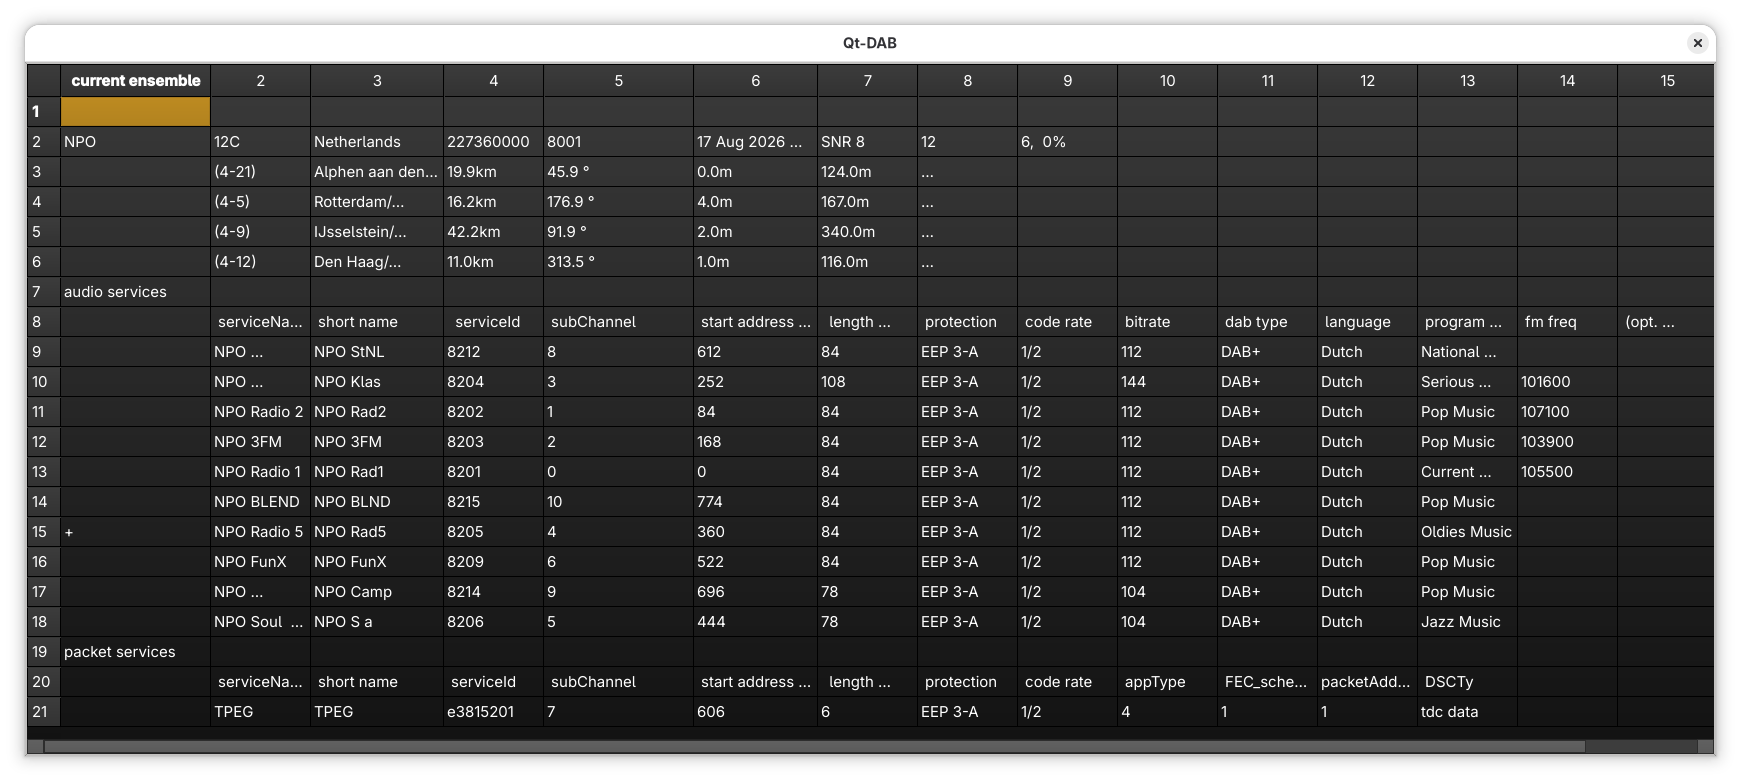
\includegraphics[width=110mm]{content-table.png}
\end{center}
\par
Clicking with the {\em right hand} mouse button on the ensemble name, again under the assumption that an ensemble was detected, starts - or stops - dumping the input samples into a file.
First a menu appears where a filename ca be specified, then a small window appears, showing the progress of the dumping.
\begin{center}
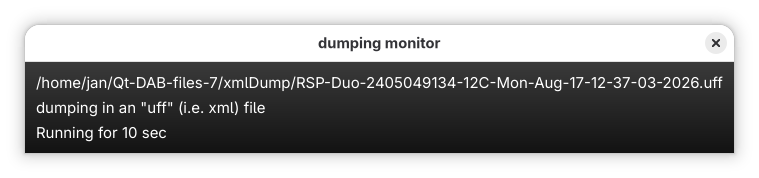
\includegraphics[width=80mm]{dump-window.png}
\end{center}
The {\em configuration and control} window contains a selector labeled
{\em input dump in xml} (set by default) that - when set tells Qt-DAB to use the xml format for dumping, if not set the PCM (i.e. ".wav") is used. Note that Qt-DAB is perfectly able to generate (and read back) PCM type files larger than 4 Gb.
\paragraph{The copyright symbol}
\begin{center}

\includegraphics[width=80mm]{topline.png}
\end{center}
The copyright symbol is written onto a clickable label, touching controls the visibility of a small window, showing some technical information and acknowledgements.
\begin{center}
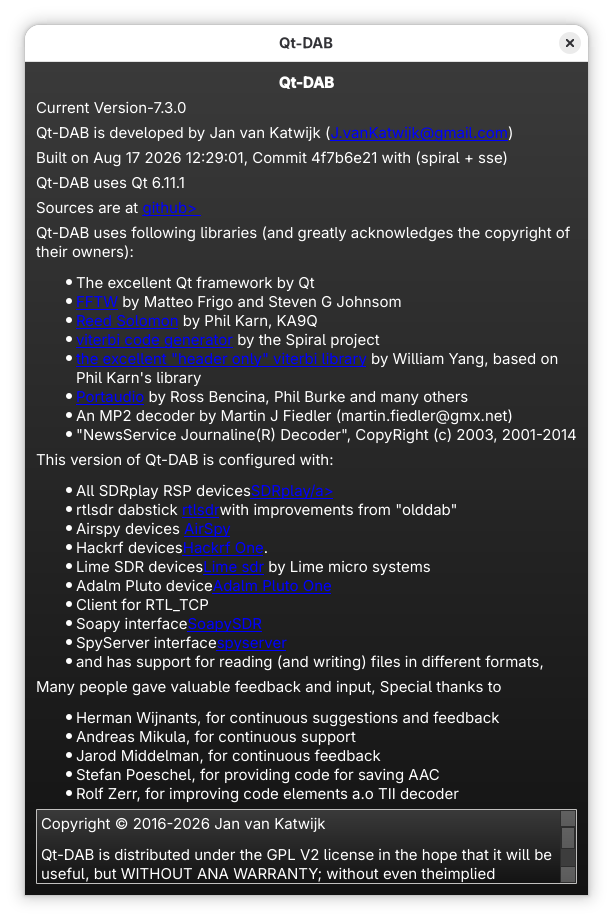
\includegraphics[width=80mm]{copyright.png}
\end{center}
\paragraph{The blue/yellow icon}
\begin{center}

\includegraphics[width=80mm]{topline.png}
\end{center}
The {\em blue/yellow} icon is shown on a clickable label, touching the label with the mouse instructs Qt-DAB to show in a separate window the directory (folder)
in which Qt-DAB stores items as slides, some dumps etc.
\begin{center}
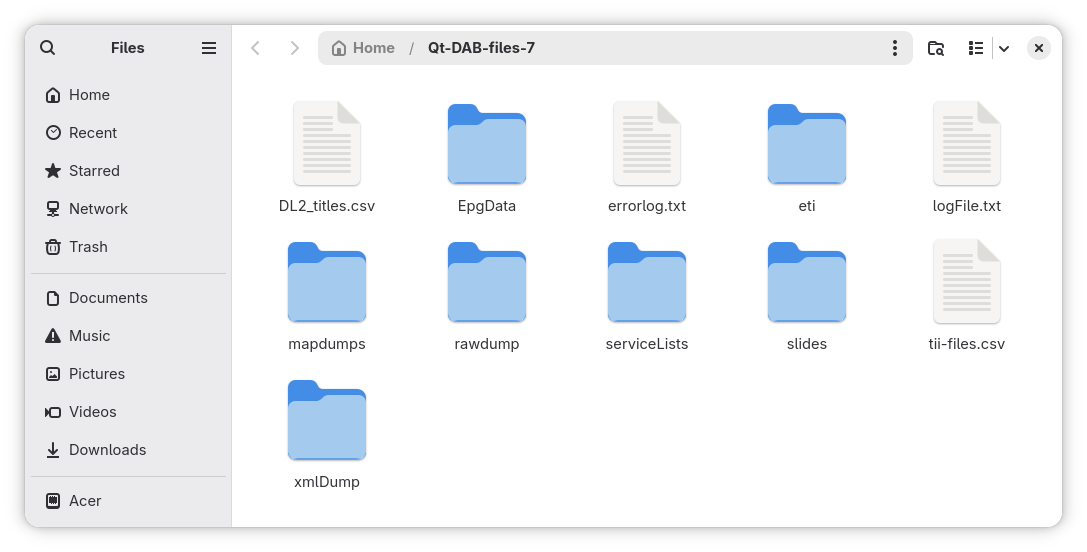
\includegraphics[width=80mm]{dabfolder.png}
\end{center}
\paragraph{The blue icon}
\begin{center}

\includegraphics[width=80mm]{topline.png}
\end{center}
The {\em small blue} icon is shown on a clickable label, touching the label with the mouse controls the visibility of a small separate window with a list of configured devices
\begin{center}
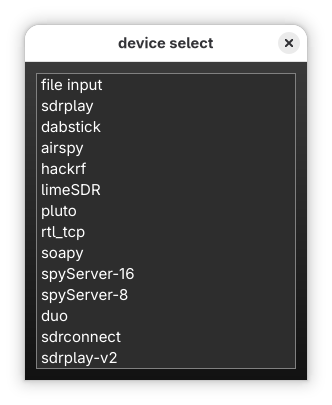
\includegraphics[width=50mm]{devicelist.png}
\end{center}
\paragraph{The SNR indicator}
\begin{center}

\includegraphics[width=80mm]{topline.png}
\end{center}
The SNR indicator at the top right of the window is displayed on a clickable label, touching it controls the visibility of a small separate window, showing the progress of the SNR in time
\begin{center}
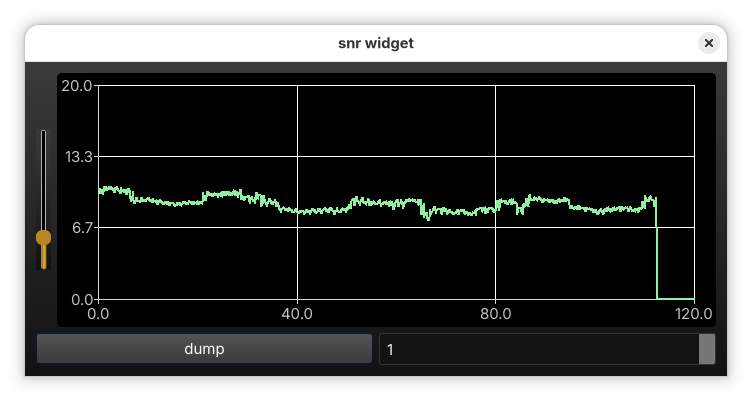
\includegraphics[width=80mm]{snr-window.png}
\end{center}
\paragraph{The list/book style style indicator}
\begin{center}
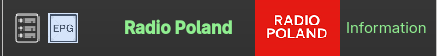
\includegraphics[width=80mm]{second-line.png}
\end{center}
The {\em list/bool style} icon on the second line is displayed on a clickable label, touching it controls the visibility of the {\em technical data}, where info on the selected audio service is displayed. Since version 7.3.0 the technical
\begin{center}
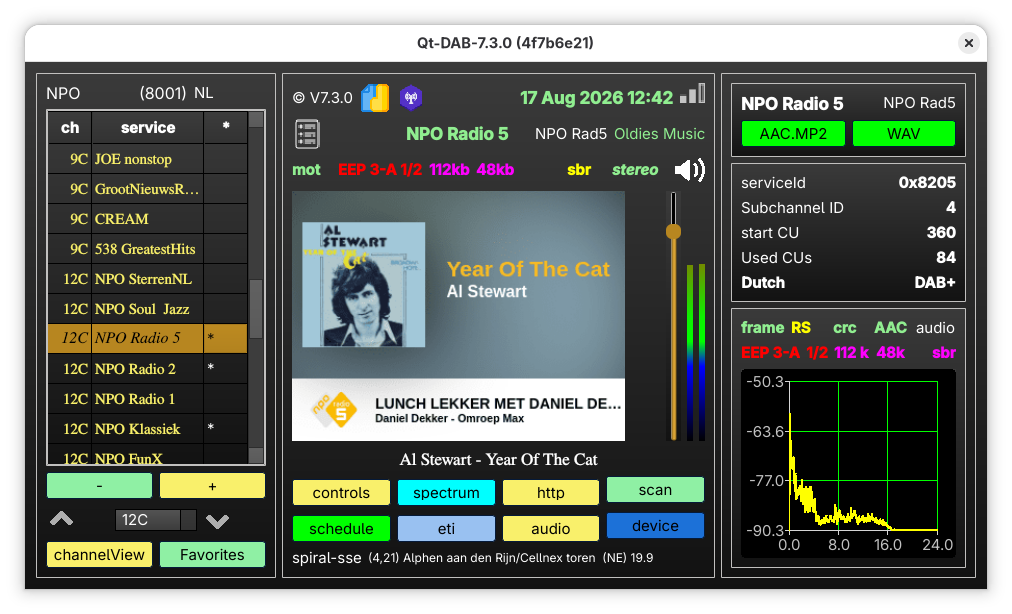
\includegraphics[width=95mm]{full-mainwindow.png}
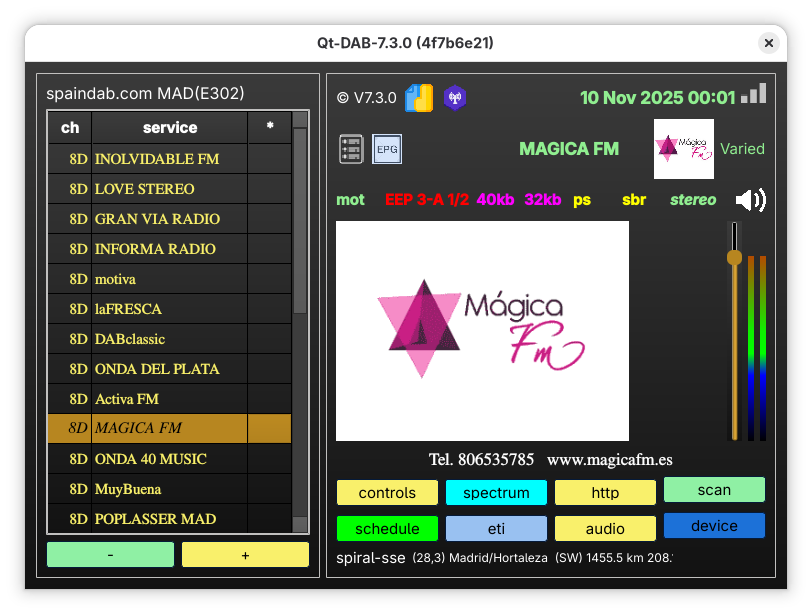
\includegraphics[width=70mm]{short-mainwindow.png}
\end{center}
data is implemented as a separate frame in the main window.
\paragraph{The EPG icon}
\begin{center}
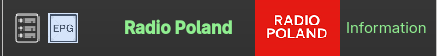
\includegraphics[width=80mm]{second-line.png}
\end{center}
The {\em EPG icon} is displayed on a clickable window. It is ONLY shown if the current ensemble contains an EPG/SPI type service. In the Netherlands, the ensembles do not contain such a service, the icon is not shown. If the icon is shown, it controls the visibility of a small window displaying potential EPG (i.e. Electronic Program Guide) data.
\begin{center}
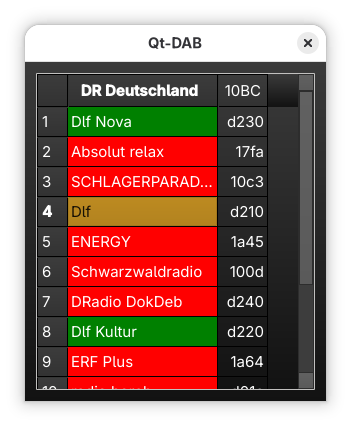
\includegraphics[width=50mm]{epg-window.png}
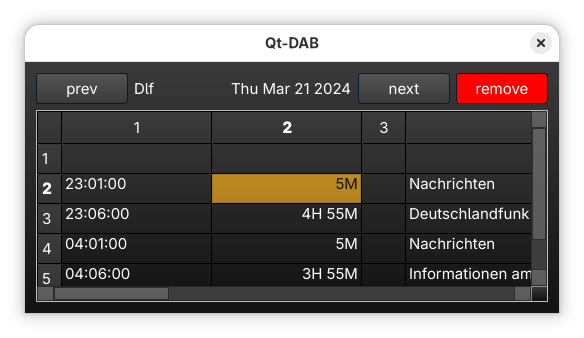
\includegraphics[width=50mm]{timetable-window.png}
\end{center}
Note that building up EPG data takes time.
\paragraph{The speaker symbol}
\begin{center}

\includegraphics[width=80mm]{third-line.png}
\end{center}
The speaker symbol shows whether or not sound is emitted. The icon itself is - as the others mentioned here - displayed on a clickable label.
\par
Touching with the {\em left hand} mouse button controls {\em muting} the audio. On clicking the audio is muted and the main window shows a counter telling the duration of muting the sound. Of course, clicking again stops muting.
\begin{center}
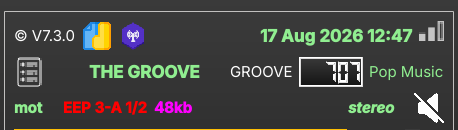
\includegraphics[width=60mm]{muting-window.png}
\end{center}
\par
When touching  with the the {\em right hand} mouse button, a small separate window shows where the (maximum) duration of muting can be set in minutes. As expected, clicking for a second time hides this window.
\begin{center}
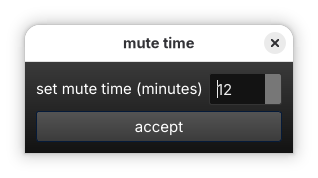
\includegraphics[width=40mm]{muting-time.png}
\end{center}
\paragraph{Touching the transmitter line}
The bottom line of the right (middle) part of the main window shows the name of one of the transmitters, detected by Qt-DAB in the current ensemble.
The text is displayed on a clickable label, touching it controls the visibility of a separate window showing details of ALL transmitters detected in the current channel.
\begin{center}
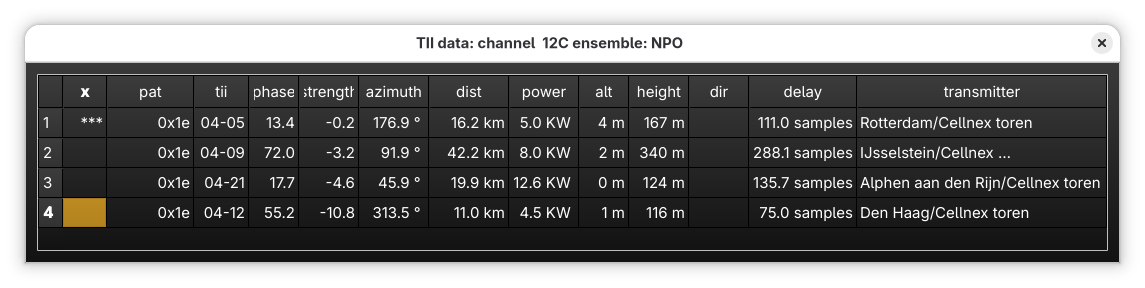
\includegraphics[width=140mm]{transmitter-window.png}
\end{center}
\paragraph{Coloring buttons}
Personally I want to have some control on the color of things, two different types of items come into mind, coloring the buttons and coloring the displays.
Both are possible, the coloring the latter is discussed elsewhere.
\begin{center}
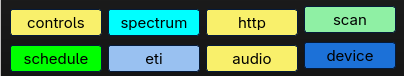
\includegraphics[width=60mm]{buttons.png}
\end{center}
For all buttons used in QT-DAB's gui (one exception), the colors can be set.
Touching with the {\em right hand} mouse button a button on the GUI shows a
color selector
\begin{center}
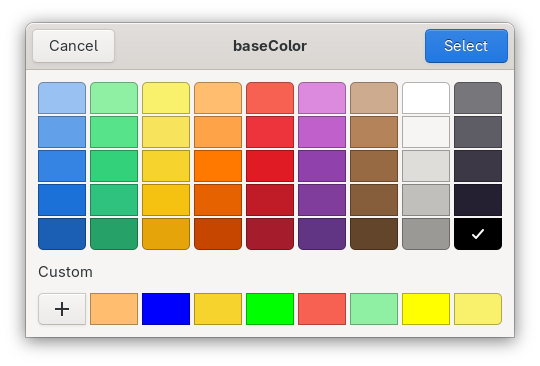
\includegraphics[width=60mm]{color-scheme.png}
\end{center}
For changing a button color the following steps have to be taken:
\begin{enumerate}
\item click with the {\em right hand} mouse button on the button;
\item select a color on the color selector, the first selection is the background color;
\item select a second color on the color selector, the second selection is the text color.
\end{enumerate}
Obviously, the color settings are kept between program invocations.
\paragraph{Disclaimer}
Qt-DAB is developed as hobby program in spare time. Being retired I do have (some) spare time and programming Qt-DAB (and my other programs) is just hobby.
It is important to notice that Qt-DAB is - both the sources as the precompiled
versions - available {\em as is}.
While it is - obviously - nice if the Qt-DAB software is useful, there are no guarantees, however. If the software does not fit your purpose, or you have
problems building an executable, recall that the Qt-DAB software is distributed in the hope that it will be useful, but WITHOUT ANY WARRANTY; without even the implied warranty of MERCHANTABILITY or FITNESS FOR A PARTICULAR PURPOSE.
See the GNU General Public License for more details.

If, however, the software seems useful and you have suggestions for improving and/or extending it, feel free to contact me, suggestions are always welcome (although no guarantees are given that they will be applied.)
\end{document}
